\documentclass[12pt]{article}

%packages
\usepackage{fancyhdr}
\usepackage[margin=1in]{geometry}
\usepackage[utf8]{inputenc}
\usepackage{listings}
\usepackage{booktabs}
\usepackage{enumitem}
\usepackage{pdfpages}
\usepackage{graphicx}
\usepackage{listings}
\usepackage{xcolor}
\usepackage{rotating}
\usepackage{subcaption}
\usepackage{float}
\usepackage{amsmath}

%fancyheadr fix
\setlength{\headheight}{15pt}

%commands to lslistings
\lstset{
    basicstyle=\ttfamily\small,
    breaklines=true,     
    breakatwhitespace=true,
    frame=single,
    numbers=left,
    numberstyle=\tiny,
    columns=fullflexible,
    keepspaces=true
}


%title info
\newcommand{\doctitle}{STA 5635 HW 9}
\newcommand{\name}{Palmer Swanson}
\newcommand{\docdate}{\today}

%document
\begin{document}

\begin{center}
    {\Large \doctitle}\\[6pt]
    {\name}\\[3pt]
    {\docdate}
\end{center}
\vspace{12pt}

\section*{Problem 1}
\begin{table}[htbp]
        \centering
        \input{../output/smallest_test_error.tex}
        \caption{Minimized x and y values for the three expressions, as well as the values of the expressions.}
        \label{tab:table_problem_1}
\end{table}

% \begin{figure}[htbp]
%     \centering 
%     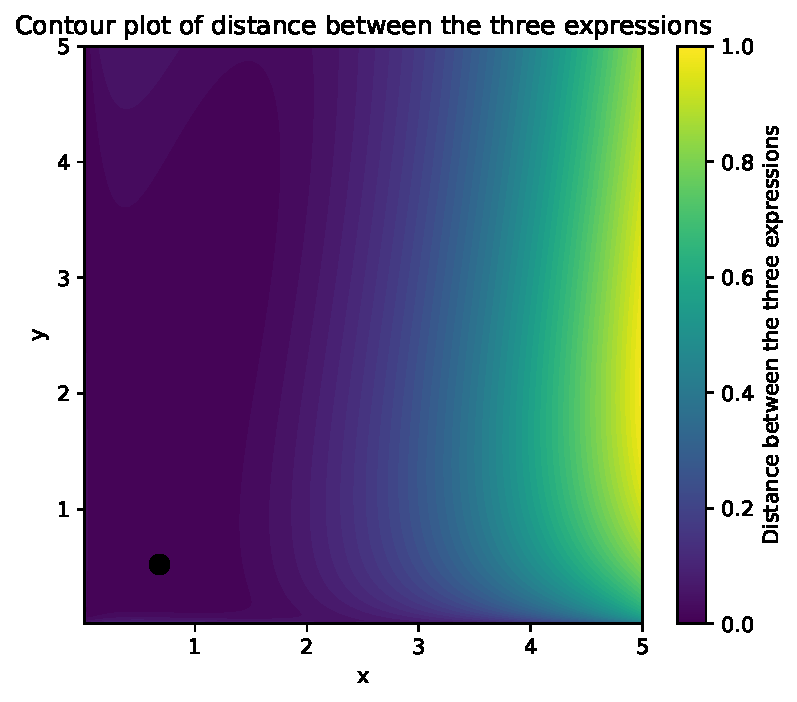
\includegraphics[width=0.7\linewidth]{../figures/contour_of_solution.pdf} 
%     \caption{Distance between the three equations and what x, y value minimizes said distance.}
% \end{figure}

\section*{Problem 2}
\subsection*{Part a}

\input{../output/viterbi_path.tex}

% \begin{figure}[htbp]
%     \centering 
%     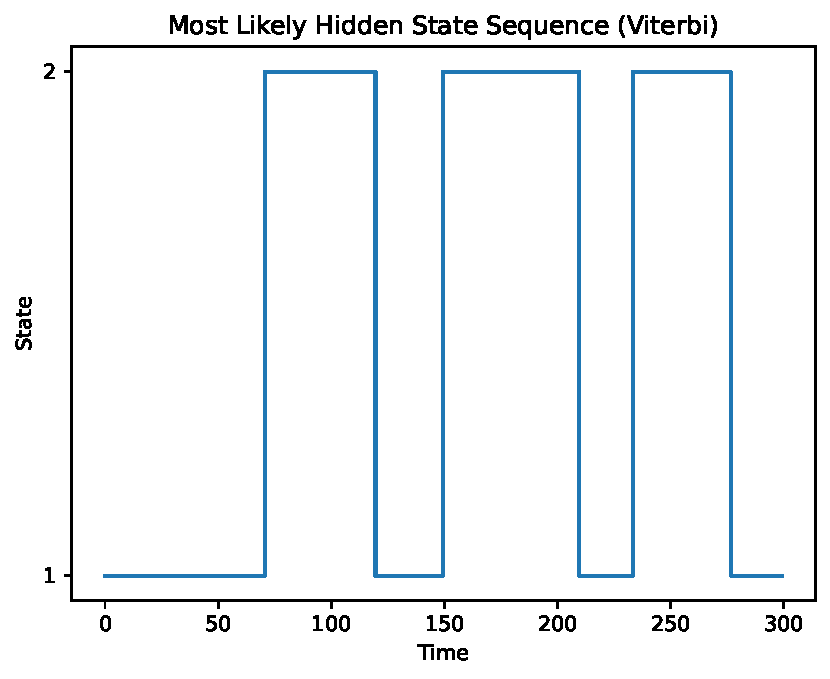
\includegraphics[width=0.7\linewidth]{../figures/state_sequence.pdf} 
%     \caption{Most likely state, Viterbi Algorithm}
% \end{figure}

\subsection*{Part b}
The ratio of alpha values at time 118: 0.4970\\
The ratio of beta values at time 118: 1.3175

\section*{Problem 3}

\input{../output/hmm_estimates.tex}

% \begin{figure}[htbp]
%     \centering 
%     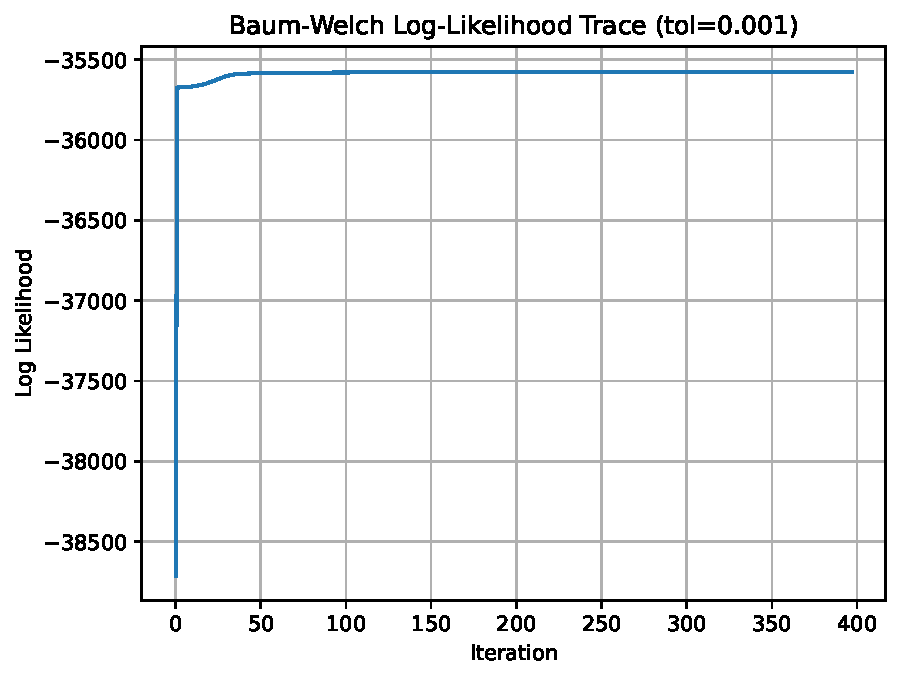
\includegraphics[width=0.7\linewidth]{../figures/log_likelihood_trace.pdf} 
%     \caption{Log Likelihood of Baum Algorithm, showing convergence.}
% \end{figure}

% \newpage
% \newpage
% %adding code
% \appendix
% \section*{Code}
% \lstinputlisting[language=Python]{../code/hw08.py}

\end{document}